\documentclass[lettersize,journal]{IEEEtran}
\usepackage{amsmath,amsfonts,amssymb}
\usepackage{array}
\usepackage{booktabs}
\usepackage{multirow}
\usepackage{graphicx}
\usepackage{textcomp}
\usepackage{stfloats}
\usepackage{url}
\usepackage{cite}
\usepackage{xcolor}
\usepackage{tikz}
\usetikzlibrary{positioning,arrows.meta,fit,calc,backgrounds}
\usepackage[hidelinks]{hyperref}
\graphicspath{{figures/}}
\hyphenation{Efficient-Net SIPaKMeD NHANES question-naire}

% ---------------------------------------------------------------- float placement
% Let LaTeX put more floats on a page and accept fuller float pages, so figures settle near the
% text that discusses them instead of queueing up at the end of the document.
\renewcommand{\topfraction}{0.92}
\renewcommand{\bottomfraction}{0.70}
\renewcommand{\textfraction}{0.06}
\renewcommand{\floatpagefraction}{0.70}
\renewcommand{\dbltopfraction}{0.92}
\renewcommand{\dblfloatpagefraction}{0.70}
\setcounter{topnumber}{3}
\setcounter{bottomnumber}{2}
\setcounter{totalnumber}{5}
\setcounter{dbltopnumber}{3}

% ---------------------------------------------------------------- notation
\newcommand{\logit}{\operatorname{logit}}
\newcommand{\pimg}{p_{\mathrm{img}}}
\newcommand{\ptab}{p_{\mathrm{tab}}}
\newcommand{\piimg}{\pi_{\mathrm{img}}}
\newcommand{\pitab}{\pi_{\mathrm{tab}}}
% ---------------------------------------------------------------- slide-grouped robustness run (filled from results/grouped_*)
\newcommand{\GTacc}{0.974}
\newcommand{\GSacc}{0.958}
\newcommand{\GSfone}{0.958}
\newcommand{\GSauc}{0.995}
\newcommand{\GSbin}{0.995}
\newcommand{\GTfone}{0.973}
\newcommand{\GTauc}{0.997}
\newcommand{\GTbin}{0.998}

\tikzset{
  box/.style={draw, rounded corners=2pt, align=center, font=\footnotesize, inner sep=3pt, minimum height=8mm, fill=white},
  data/.style={box, fill=gray!10},
  model/.style={box, line width=0.9pt},
  op/.style={box, dashed},
  arr/.style={-{Stealth[length=2mm]}, line width=0.6pt},
}

\begin{document}

\title{Calibrated Any-Modality Fusion of Unpaired Cytology and Questionnaire Experts for Cervical Cancer Screening Support}

\author{Author One, Author Two, Author Three, and Author Four
\thanks{Manuscript received XX; revised XX. (Corresponding author: Author One.)}
\thanks{The authors are with MUICT RAS (affiliation to be completed).}}

\markboth{IEEE Journal of Biomedical and Health Informatics}%
{Calibrated Any-Modality Fusion of Unpaired Cytology and Questionnaire Experts}

\maketitle

\begin{abstract}
Cervical screening weighs cellular morphology together with infection risk, yet public data sets never pair a cytology image with a risk questionnaire from the same woman, so joint multimodal models cannot be trained. We present a decision-level framework that fuses two independently trained experts without paired data. A cytology expert, an EfficientNet-B4 teacher distilled into a four-times smaller EfficientNet-B0 student, classifies five Pap-smear cell types with 96.4\% test accuracy, and 95.8\% when whole slides are held out. A questionnaire expert estimates high-risk human papillomavirus infection from 31 items in 12,634 women from seven national survey cycles; calibrated logistic regression reached an area under the receiver operating characteristic curve of 0.687 with an expected calibration error of 0.007. The fusion rule removes each expert's training prevalence, converts infection risk into a pre-test probability of abnormal cytology through an epidemiological link, and treats the image as a likelihood ratio; split-conformal prediction allows abstention. On a semi-synthetic cohort that pairs real held-out records through a latent infection and cytology state matched to a large screening trial, the unpaired fusion matched a stacking model trained on paired data in all 56 scenarios and never underperformed the image alone, whereas naive averaging lowered discrimination in most of them. At a screening prevalence of 7.1\%, re-anchoring cut the calibration error of a moderately accurate image expert from 0.176 to 0.004. Discrimination gains were small and appeared only when image evidence was uncertain. The framework offers calibrated, any-modality screening support without paired training data.
\end{abstract}

\begin{IEEEkeywords}
Cervical cancer screening, multimodal fusion, missing modality, probability calibration, prior shift, knowledge distillation, conformal prediction, human papillomavirus, Pap-smear cytology, explainable AI.
\end{IEEEkeywords}

%% =====================================================================
\section{Introduction}
\IEEEPARstart{C}{ervical} cancer remains one of the most common cancers in women worldwide, with most deaths occurring where routine screening and timely diagnosis are limited \cite{WHO_cervical_cancer}. Persistent infection with a high-risk human papillomavirus (HPV) genotype is a necessary cause of the disease \cite{walboomers1999hpv}, and screening programmes therefore combine two complementary views of a woman's risk: HPV testing, which measures infection, and cytology, which measures the cellular changes the infection produces \cite{WHO_screening_guideline}. A decision-support tool that could weigh a woman's infection risk together with the appearance of her cells would mirror this clinical reasoning.

Artificial intelligence already performs strongly on each view separately. Convolutional networks classify Pap-smear cells with high in-distribution accuracy \cite{zhang2017deeppap,tan2024cervical,youneszade2023deep}, and machine-learning models estimate risk from questionnaire and clinical variables \cite{fernandes2017cervical,sun2022stacking,chadaga2022predicting}. Multimodal models that combine images with clinical variables have shown gains in related cervical tasks \cite{das2026topoticerv,wang2025cervipro,sha2024cervifusionnet}, and multimodal biomedical AI is an active direction more broadly \cite{acosta2022multimodal,baltrusaitis2019multimodal}.

Two obstacles prevent such a combined tool from being built with public data. First, the modalities are \emph{unpaired}. Cytology image collections such as SIPaKMeD \cite{plissiti2018sipakmed} and Herlev \cite{jantzen2005herlev} carry no patient-level risk information, while risk-factor cohorts such as the U.S. National Health and Nutrition Examination Survey (NHANES) \cite{nhanes} carry no images. Joint-training and missing-modality methods \cite{havaei2016hemis,yao2024drfuse,wu2026deep} still need at least some patients observed in both modalities to learn how the modalities interact. Second, the two experts answer \emph{different questions} under \emph{different prevalences}. A questionnaire model predicts HPV infection; a cytology model predicts cellular abnormality; and each is trained on a class mix that differs from the one a screening clinic sees. Naively averaging their outputs mixes two endpoints and inherits two mismatched priors, which, as we show, lowers discrimination and badly miscalibrates the output.

This paper develops and evaluates a decision-level framework that fuses two independently trained experts without paired data. Its central operator, which we call CO-PRIOR, removes each expert's training prior, re-anchors the outputs to the deployment prevalence \cite{saerens2002adjusting}, converts infection risk into a pre-test probability of abnormal cytology through an explicit epidemiological link, and combines it with the image evidence as a likelihood ratio. The same rule returns the correct single-expert output when either modality is missing, and a split-conformal gate \cite{vovk2005algorithmic,angelopoulos2023conformal} lets the system defer uncertain cases. Because no real patient has both inputs, we evaluate the fused system on a semi-synthetic cohort in which each simulated woman is assigned a real held-out questionnaire record and a real held-out cell image through a latent infection-and-cytology state matched to the ATHENA screening trial \cite{wright2012athena}.

The contributions are:
\begin{enumerate}
\item Two calibrated, reproducible experts evaluated under leakage-aware protocols: a distilled cytology classifier that matches its teacher with four times fewer parameters, and an HPV-risk questionnaire model trained on 12,634 NHANES participants with in-fold imputation, class weighting instead of synthetic oversampling, and nested isotonic calibration.
\item CO-PRIOR fusion: a closed-form, training-free rule that combines unpaired experts with different endpoints and priors, reduces to the appropriate single-expert output under missing modalities, and is paired with conformal abstention.
\item A semi-synthetic paired-cohort protocol built from real held-out records and trial-matched margins, used to measure the fused system across link strength, image quality, link misspecification, missing inputs and abstention. The unpaired fusion matches a model trained on paired data, naive fusion is harmful, and the dominant practical benefit is calibration at screening prevalence.
\item Transparent reporting of the image evaluation, including a fixed test set, a slide-grouped robustness analysis that quantifies overlap between full-field and cropped images in the standard SIPaKMeD split, and visual (Grad-CAM) and tabular (SHAP, permutation importance) explanations.
\end{enumerate}

Fig.~\ref{fig:framework} summarises the system.

\begin{figure*}[t]
\centering
\resizebox{0.98\textwidth}{!}{%
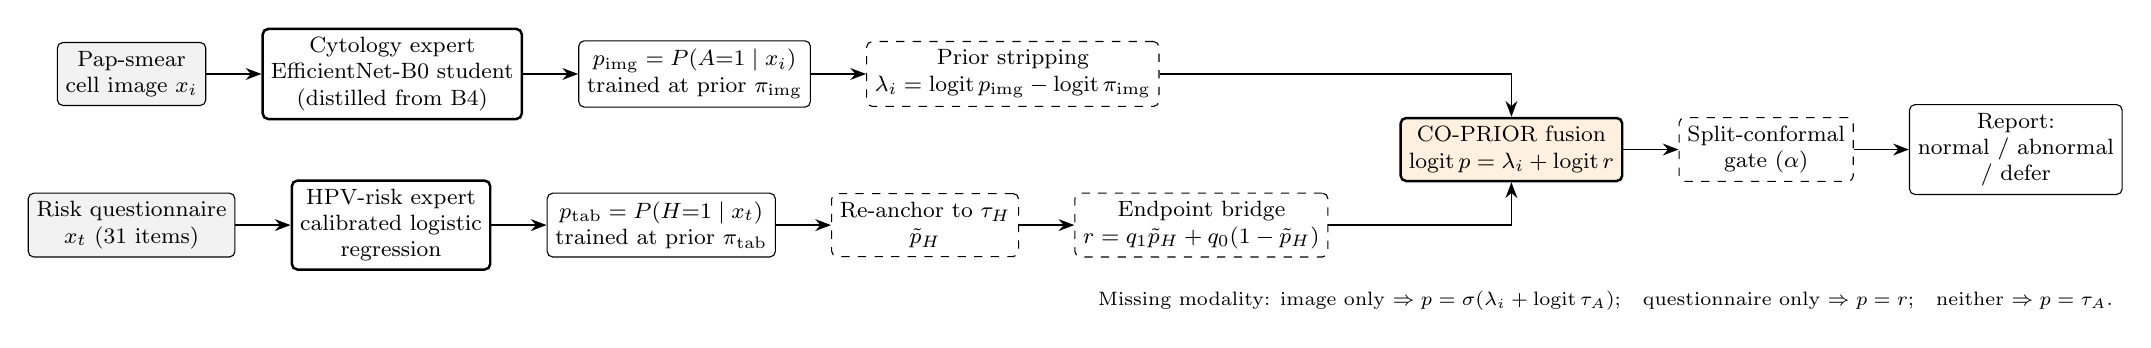
\begin{tikzpicture}[node distance=5mm and 7mm]
  \node[data] (img) {Pap-smear\\cell image $x_i$};
  \node[model, right=of img] (ce) {Cytology expert\\EfficientNet-B0 student\\(distilled from B4)};
  \node[box, right=of ce] (pi) {$\pimg = P(A{=}1\mid x_i)$\\trained at prior $\piimg$};
  \node[op, right=of pi] (lr) {Prior stripping\\$\lambda_i = \logit\pimg - \logit\piimg$};
  \node[data, below=11mm of img] (tab) {Risk questionnaire\\$x_t$ (31 items)};
  \node[model, right=of tab] (he) {HPV-risk expert\\calibrated logistic\\regression};
  \node[box, right=of he] (pt) {$\ptab = P(H{=}1\mid x_t)$\\trained at prior $\pitab$};
  \node[op, right=of pt] (an) {Re-anchor to $\tau_H$\\$\tilde p_H$};
  \node[op, right=of an] (br) {Endpoint bridge\\$r = q_1\tilde p_H + q_0(1-\tilde p_H)$};
  \path let \p1 = (br.east), \p2 = (lr.east), \p3 = (br.east) in
        node[model, fill=orange!12, anchor=west] (fu) at (\x1+9mm, {(\y2+\y3)/2}) {CO-PRIOR fusion\\$\logit p = \lambda_i + \logit r$};
  \node[op, right=of fu] (cp) {Split-conformal\\gate ($\alpha$)};
  \node[box, right=of cp] (out) {Report:\\normal / abnormal\\/ defer};
  \draw[arr] (img) -- (ce); \draw[arr] (ce) -- (pi); \draw[arr] (pi) -- (lr);
  \draw[arr] (tab) -- (he); \draw[arr] (he) -- (pt); \draw[arr] (pt) -- (an); \draw[arr] (an) -- (br);
  \draw[arr] (lr.east) -| (fu.north); \draw[arr] (br.east) -| (fu.south);
  \draw[arr] (fu) -- (cp); \draw[arr] (cp) -- (out);
  \node[font=\scriptsize, anchor=north east] at ($(out.south east)+(0,-11mm)$)
     {Missing modality: image only $\Rightarrow p=\sigma(\lambda_i+\logit\tau_A)$;\quad questionnaire only $\Rightarrow p=r$;\quad neither $\Rightarrow p=\tau_A$.};
\end{tikzpicture}}
\caption{Overview of the framework. Two experts are trained on separate, unpaired data sets and are never retrained jointly. The cytology expert predicts cellular abnormality $A$; the questionnaire expert predicts high-risk HPV infection $H$. CO-PRIOR removes each expert's training prior, maps infection risk to a pre-test probability of abnormal cytology through the link probabilities $q_1=P(A{=}1\mid H{=}1)$ and $q_0=P(A{=}1\mid H{=}0)$, and adds the image evidence as a log-likelihood ratio. A split-conformal gate defers cases whose prediction set is not a single class.}
\label{fig:framework}
\end{figure*}

%% =====================================================================
\section{Related Work}

\subsection{Clinical risk factors and machine-learning risk prediction}
Before deep learning, cervical cancer prediction relied mainly on traditional machine-learning algorithms trained on structured clinical information and patient risk factors. Early studies compared numerous supervised learners, and ensembles of several classifiers generally outperformed individual models, with tree-based methods achieving high accuracy on the UCI Cervical Cancer Risk Factors data set \cite{fernandes2017cervical}. Imputation strategies ranging from mean substitution to $k$-nearest-neighbour and support-vector-machine imputation have been used to reconstruct missing clinical information before training \cite{karamti2023improvingpr,munshi2024novel}. Severe class imbalance is commonly addressed with oversampling such as SMOTE, SMOTE-Tomek links, ADASYN and random oversampling, often combined with outlier detection \cite{ijaz2020data}, and voting, boosting and stacking ensembles have been investigated to improve performance \cite{sun2022stacking,chadaga2022predicting}. When oversampling or imputation is fitted before the data are split, however, synthetic or imputed information leaks into the evaluation folds; we therefore fit every preprocessing step inside the cross-validation loop and use class weighting instead of synthetic oversampling.

\subsection{Deep learning for cervical cytology}
Deep learning has advanced cervical cancer diagnosis by learning features directly from images. DeepPap was among the first studies to apply deep convolutional networks and transfer learning to cervical cell classification, showing that ImageNet-pretrained representations adapt effectively to cytology despite limited annotated data \cite{zhang2017deeppap}. A comparison of thirteen pretrained architectures found DenseNet-201 to perform best on the Herlev data set \cite{tan2024cervical}. Whole-slide frameworks combine patch-level networks with slide-level aggregation and have been evaluated on independent private cohorts \cite{yan2025deep}, and Swin-Transformer ensembles have been applied to colposcopy images \cite{himabindu2025swin}. Reviews highlight persistent challenges: limited data-set diversity, class imbalance, lack of external validation and difficult clinical translation \cite{vallescoral2026review,youneszade2023deep}.

\subsection{Foundation models}
These limitations have motivated pathology foundation models that learn transferable representations from very large collections. UniCAS is a cervical cytology foundation model pretrained with self-supervision on more than 48,000 whole-slide images and evaluated on screening, candidiasis detection and subtype diagnosis \cite{jiang2026unicas}. General-purpose pathology models such as UNI \cite{chen2024uni}, the vision-language model CONCH \cite{lu2024visual}, the multimodal slide-level model TITAN \cite{ding2025titan} and the gigapixel model Prov-GigaPath \cite{xu2024provgigapath} provide representations that may benefit cervical pathology when labelled data are scarce.

\subsection{Multimodal learning for cervical cancer}
Clinical decisions also draw on information outside the image, such as age, HPV status, smoking history, parity and previous findings. TopotiCerv integrates acetowhite colposcopic images with clinical findings for lesion classification \cite{das2026topoticerv}; Wang \emph{et al.} combined pre- and post-treatment CT, radiomic features and clinical variables to predict disease-free survival after radiotherapy \cite{wang2025cervipro}; CerviFusionNet fuses original, acetic-acid and iodine colposcopic images through a hybrid CNN--Transformer--GRU network \cite{sha2024cervifusionnet}; radiomic and deep features have been combined for lesion detection with external validation \cite{niu2025hybridfeatu}; and graph neural networks have fused segmented regions within colposcopy images \cite{chatterjee2025multi}. Incomplete patient information is a practical challenge, addressed through feature completion, modality hallucination, distillation and modality-invariant representations \cite{wu2026deep,havaei2016hemis,yao2024drfuse}. All of these approaches learn cross-modal interactions from patients observed in more than one modality; none addresses the case in which the modalities come from entirely disjoint populations.

\subsection{Data-set heterogeneity and label harmonisation}
Public cytology collections, including Herlev \cite{jantzen2005herlev}, SIPaKMeD \cite{plissiti2018sipakmed}, CRIC \cite{rezende2021cric}, APACC \cite{kupas2024apacc} and HiCervix \cite{cai2024hicervix}, differ in acquisition, staining, magnification, segmentation, class distributions and annotation schemes \cite{coskun2026robust}, and newer liquid-based cytology sets add further diversity \cite{hussain2020liquidbased}. The Bethesda System provides a clinically established vocabulary for cytology reporting that supports medically justified harmonisation of heterogeneous labels \cite{solomon2002bethesda,nayar2015bethesda}; we use it to collapse the five SIPaKMeD cell types into the binary normal/abnormal decision that the fusion consumes. Large-scale validation, such as the multicentre retrospective, prospective and randomised evaluation reported by Wang \emph{et al.} \cite{wang2024aiccs}, remains the benchmark for trustworthy screening AI. Explainability methods, including SHAP feature attribution, LIME and Grad-CAM localisation, are increasingly reported alongside performance \cite{vallescoral2026review}.

\subsection{Decision-level fusion, calibration and uncertainty}
Classifier-combination rules such as the product and sum rules \cite{kittler1998combining} assume experts that output posteriors for the \emph{same} label under the \emph{same} prior. When class priors differ between training and deployment, posteriors can be corrected by Bayes' rule without retraining \cite{saerens2002adjusting,lipton2018labelshift}. Modern networks are frequently miscalibrated \cite{guo2017calibration}, and Platt scaling \cite{platt1999probabilistic} and isotonic regression \cite{zadrozny2002transforming} are standard remedies. Conformal prediction offers distribution-free coverage guarantees \cite{vovk2005algorithmic,angelopoulos2023conformal} and has recently been validated for cervical atypia classification \cite{hagos2026conformal}; cytologist-in-the-loop systems show the clinical value of deferring uncertain cells to experts \cite{xue2023arcytologist}.

\subsection{Research gaps}
Three gaps motivate this work. (i) Multimodal cervical models require patients observed in several modalities, whereas the largest public image and risk-factor resources are disjoint. (ii) Experts trained on different endpoints (infection versus cytological abnormality) and different class mixes are rarely combined in a way that respects both differences, so their fused outputs are neither well-ranked nor calibrated at screening prevalence. (iii) Evaluations seldom report calibration, abstention and behaviour under missing inputs, which are central to safe decision support. We address these gaps with a prior-aware, endpoint-aware decision-level fusion evaluated on a trial-anchored semi-synthetic cohort; systematic cross-data-set validation of the image expert under Bethesda harmonisation is left to future work.

%% =====================================================================
\section{Materials}

\subsection{Cytology images: SIPaKMeD}
SIPaKMeD \cite{plissiti2018sipakmed} contains conventional Pap-smear images from five cell categories: dyskeratotic and koilocytotic cells, which are abnormal and correspond to the squamous intraepithelial lesion spectrum of the Bethesda System \cite{solomon2002bethesda}; metaplastic cells, which are benign; and parabasal and superficial-intermediate cells, which are normal. The release contains 966 full-field images, each showing a cell cluster, and 4,049 single cells cropped from those fields, for 5,015 images in total (1,036 dyskeratotic, 1,063 koilocytotic, 1,064 metaplastic, 895 parabasal and 957 superficial-intermediate). Classes are nearly balanced (largest-to-smallest ratio 1.19), and abnormal cells make up 41.8\% of the collection, a figure that matters later because it is the prior the cytology expert learns. Because every cropped cell is cut from one of the full-field images, the two image types are not independent; we return to this in Section~\ref{sec:split}.

\subsection{Risk questionnaires: NHANES}
The questionnaire expert uses NHANES \cite{nhanes}, a nationally representative U.S. survey. We pooled the seven cycles from 2003--2004 to 2015--2016 in which women aged 18--59 provided a self-collected vaginal swab genotyped for HPV, and merged the demographic (DEMO), sexual-behaviour (SXQ), reproductive-health (RHQ), smoking (SMQ), immunisation (IMQ) and herpes-serology (HSV) files by participant identifier. The target is infection with any of 14 high-risk genotypes (16, 18, 31, 33, 35, 39, 45, 51, 52, 56, 58, 59, 66, 68). The cohort comprises 12,634 women (mean age $37.1\pm12.3$ years), of whom 3,103 (24.6\%) were positive; prevalence fell from 29.1\% in 2005--2006 to 20.4\% in 2015--2016. Table~\ref{tab:features} lists the 31 features: 28 questionnaire or laboratory items and three engineered exposure rates. The item ``ever told by a doctor that you had HPV'' was excluded because it is a self-report of the target. Several sexual-behaviour items were introduced only in 2009, so missingness ranges from 0\% to 59\%. Infection prevalence follows the gradients expected from HPV epidemiology, which supports the plausibility of the cohort: it falls from 36\% in women aged 18--24 to 17\% at 50--59, and rises from 9\% in women with at most one lifetime male partner to 35\% in those with fifteen or more.

\begin{table}[t]
\caption{Questionnaire Features (31) of the HPV-Risk Expert}
\label{tab:features}
\centering\footnotesize
\setlength{\tabcolsep}{3pt}
\begin{tabular}{@{}p{0.23\columnwidth}p{0.73\columnwidth}@{}}
\toprule
Domain & Features \\
\midrule
Demographics & age; race/ethnicity; education; marital status; income-to-poverty ratio \\
Sexual behaviour & ever had sex; age at first sex; age at first oral sex; ever oral sex; ever anal sex; lifetime partners; partners in past 12 months; lifetime vaginal partners; lifetime oral partners; condomless sex in past 12 months; new partner in past 12 months; sexual orientation \\
STI history & genital herpes; gonorrhoea; chlamydia; genital warts \\
Reproductive & age at menarche; ever pregnant; number of pregnancies \\
Smoking & $\geq$100 cigarettes in lifetime; smoking status (never/former/current) \\
Vaccination & ever received HPV vaccine \\
Serology & herpes simplex virus type-2 antibody \\
Engineered & years sexually active; partners per active year; pregnancies per active year \\
\bottomrule
\end{tabular}
\end{table}

\subsection{Screening-trial margins}
To build realistic synthetic patients we use the baseline results of the ATHENA trial \cite{wright2012athena}, which enrolled 47,208 U.S. women aged 21 years or older undergoing routine screening: 12.6\% were positive for high-risk HPV and 7.1\% had abnormal cytology. These two margins fix the prevalence of infection and of cytological abnormality in the synthetic cohort (Section~\ref{sec:synthetic}).

\subsection{Ethics}
All data are public and de-identified. NHANES protocols were approved by the National Center for Health Statistics Research Ethics Review Board with written informed consent from participants; SIPaKMeD is released for research use. No new data were collected.

%% =====================================================================
\section{Methods}

\subsection{Problem formulation}
Let $A\in\{0,1\}$ denote cytological abnormality and $H\in\{0,1\}$ high-risk HPV infection. The cytology expert maps a cell image $x_i$ to $\pimg=\hat P(A{=}1\mid x_i)$ and was trained on data with abnormality prevalence $\piimg$. The questionnaire expert maps answers $x_t$ to $\ptab=\hat P(H{=}1\mid x_t)$ and was trained with infection prevalence $\pitab$. No woman is observed with both $x_i$ and $x_t$. At deployment the clinic screens a population with infection prevalence $\tau_H$ and abnormality prevalence $\tau_A$, and the task is to output a calibrated $P(A{=}1\mid x_i,x_t)$, or the best available estimate when one input is missing, together with an option to defer.

\subsection{Cytology expert}
\label{sec:image}
\emph{Architecture.} The teacher is an EfficientNet-B4 \cite{tan2019efficientnet} initialised with ImageNet weights \cite{deng2009imagenet}, followed by global average pooling, batch normalisation, a 512-unit ReLU layer, dropout (0.5) and a five-way softmax. Inputs are resized to $380\times380$ pixels. Training-time augmentation applies random horizontal and vertical flips, rotations of up to $\pm72^\circ$ and zoom of $\pm10\%$.

\emph{Two-stage training.} In stage~1 the backbone is frozen and the head is trained with Adam (learning rate $10^{-3}$) for up to 30 epochs with class weights, early stopping on validation loss (patience 8) and learning-rate reduction by $0.3$ on plateau (patience 4, floor $10^{-6}$). In stage~2 the whole network is unfrozen and fine-tuned with Adam ($10^{-5}$) for up to 50 epochs (early-stopping patience 6). A batch size of 8 was used for fine-tuning to fit the 16~GB GPU.

\emph{Knowledge distillation.} A student EfficientNet-B0 with the same head (dropout 0.3) is trained from the frozen teacher \cite{hinton2015distilling} with
\begin{equation}
\mathcal L = \alpha\,\mathrm{CE}(y,s) + (1-\alpha)\,\mathrm{KL}\!\left(\sigma(t/T)\,\|\,\sigma(s/T)\right),
\label{eq:kd}
\end{equation}
where $t$ and $s$ are the teacher and student output vectors, $\sigma$ is the softmax, $\alpha=0.1$ and $T=4$, using Adam ($5\times10^{-5}$) for up to 40 epochs with early stopping on validation accuracy (patience 8). In our implementation $t$ and $s$ are the softmax outputs of the two networks, so the temperature acts on probabilities rather than logits.

\emph{Bethesda collapse.} For fusion, the five-class output is reduced to the probability of an abnormal cell, $\pimg = P(\text{dyskeratotic}) + P(\text{koilocytotic})$.

\emph{Data splits.}
\label{sec:split}
\emph{Protocol~A (primary).} Following common practice with this data set, all 5,015 images were split at random at the file level (seed 42) into 70\% training (3,511), 20\% validation (1,000) and 10\% test (504). Keras reshuffles the held-out data on each pass, so we reconstructed the identical file-level split and fixed the test set as a defined list of 504 files; no held-out file was used for gradient updates. Because cropped cells and their parent full-field images can fall on different sides of this split, 404 of the 414 cropped test cells come from a slide that also contributed images to training. \emph{Protocol~B (robustness).} To measure the effect of this overlap, we repeated the full teacher--student recipe on the 4,049 cropped cells only, assigning whole source slides within each class to training, validation and test (70/20/10), so that no test cell shares a slide with any training cell (2,819/851/379 cells).

\subsection{HPV-risk expert}
\label{sec:tabular}
Fig.~\ref{fig:pipelines} (bottom) summarises the pipeline. Six classifier families were compared: logistic regression, $k$-nearest neighbours ($k=5$), random forest \cite{breiman2001random}, extremely randomised trees \cite{geurts2006extremely}, LightGBM \cite{ke2017lightgbm} and XGBoost \cite{chen2016xgboost} (600 trees each where applicable). Class imbalance was handled by class weights (scale-positive-weight 3.07 for XGBoost) rather than synthetic oversampling. Median imputation, and standardisation for the linear and nearest-neighbour models, were fitted inside each training fold. All models were evaluated with stratified five-fold cross-validation (seed 42) using out-of-fold predictions, with 95\% confidence intervals from 1,000 bootstrap resamples \cite{efron1994bootstrap}. The family with the highest AUROC was calibrated with isotonic regression \cite{zadrozny2002transforming} in a nested three-fold scheme, so every calibrated probability is also out-of-fold. Explanations were obtained from permutation importance (mean AUROC drop over five permutations on held-out folds) and TreeSHAP \cite{lundberg2017unified,lundberg2020local} on a 200-tree random forest for 800 randomly selected participants. All tabular models used scikit-learn \cite{pedregosa2011scikit}.

\begin{figure*}[t]
\centering
\resizebox{0.98\textwidth}{!}{%
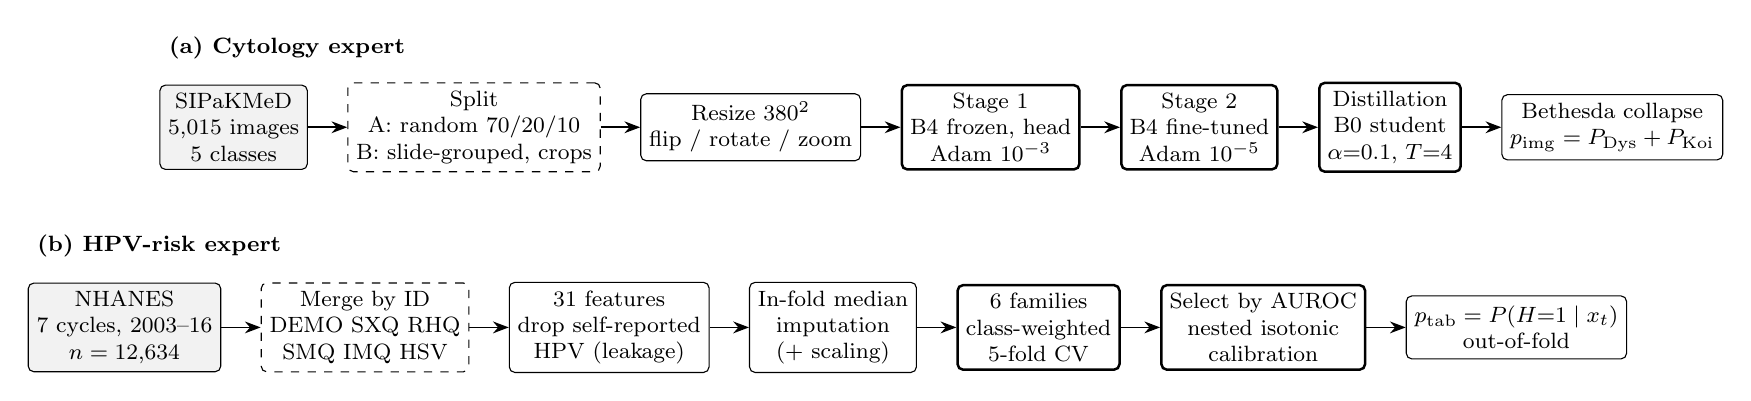
\begin{tikzpicture}[node distance=4mm and 5mm]
  \node[font=\footnotesize\bfseries, anchor=west] (la) {(a) Cytology expert};
  \node[data, below=2mm of la.south west, anchor=north west] (s0) {SIPaKMeD\\5,015 images\\5 classes};
  \node[op, right=of s0] (s1) {Split\\A: random 70/20/10\\B: slide-grouped, crops};
  \node[box, right=of s1] (s2) {Resize $380^2$\\flip / rotate / zoom};
  \node[model, right=of s2] (s3) {Stage 1\\B4 frozen, head\\Adam $10^{-3}$};
  \node[model, right=of s3] (s4) {Stage 2\\B4 fine-tuned\\Adam $10^{-5}$};
  \node[model, right=of s4] (s5) {Distillation\\B0 student\\$\alpha{=}0.1,\,T{=}4$};
  \node[box, right=of s5] (s6) {Bethesda collapse\\$\pimg=P_{\rm Dys}+P_{\rm Koi}$};
  \foreach \a/\b in {s0/s1,s1/s2,s2/s3,s3/s4,s4/s5,s5/s6} \draw[arr] (\a) -- (\b);
  \node[font=\footnotesize\bfseries, anchor=west, below=7mm of s0.south west] (lb) {(b) HPV-risk expert};
  \node[data, below=2mm of lb.south west, anchor=north west] (t0) {NHANES\\7 cycles, 2003--16\\$n=12{,}634$};
  \node[op, right=of t0] (t1) {Merge by ID\\DEMO SXQ RHQ\\SMQ IMQ HSV};
  \node[box, right=of t1] (t2) {31 features\\drop self-reported\\HPV (leakage)};
  \node[box, right=of t2] (t3) {In-fold median\\imputation\\(+ scaling)};
  \node[model, right=of t3] (t4) {6 families\\class-weighted\\5-fold CV};
  \node[model, right=of t4] (t5) {Select by AUROC\\nested isotonic\\calibration};
  \node[box, right=of t5] (t6) {$\ptab = P(H{=}1\mid x_t)$\\out-of-fold};
  \foreach \a/\b in {t0/t1,t1/t2,t2/t3,t3/t4,t4/t5,t5/t6} \draw[arr] (\a) -- (\b);
\end{tikzpicture}}
\caption{Training pipelines of the two experts. (a) Cytology: two-stage EfficientNet-B4 teacher training followed by distillation into an EfficientNet-B0 student, evaluated under a random file-level split (Protocol~A) and a slide-grouped split of cropped cells (Protocol~B). (b) HPV risk: NHANES files are merged, the target self-report is excluded, and all preprocessing is fitted within cross-validation folds before model selection and nested calibration. Bold borders mark trained models.}
\label{fig:pipelines}
\end{figure*}

\subsection{CO-PRIOR fusion}
\label{sec:coprior}
\emph{Prior stripping and re-anchoring.} If an expert is calibrated for prior $\pi$ and only the class prior changes between training and deployment (label shift), Bayes' rule gives the posterior at a new prior $\tau$ as \cite{saerens2002adjusting}
\begin{equation}
\logit \tilde p = \logit p - \logit \pi + \logit \tau .
\label{eq:anchor}
\end{equation}
The difference $\lambda = \logit p - \logit\pi$ is the expert's log-likelihood ratio: the evidence contributed by the input, free of the prior.

\emph{Endpoint bridge.} The questionnaire expert predicts infection, not abnormality. After re-anchoring $\ptab$ to the deployment infection prevalence $\tau_H$ with \eqref{eq:anchor}, giving $\tilde p_H$, the pre-test probability of abnormal cytology is
\begin{equation}
r(x_t) = q_1\,\tilde p_H + q_0\,(1-\tilde p_H),
\label{eq:bridge}
\end{equation}
with $q_h = P(A{=}1\mid H{=}h)$. Given the deployment margins $\tau_H$ and $\tau_A$ and an odds ratio $\mathrm{OR}$ linking infection to abnormal cytology, $q_1$ and $q_0$ are the unique solution of $\tau_H q_1 + (1-\tau_H) q_0 = \tau_A$ and $q_1(1-q_0)/[q_0(1-q_1)] = \mathrm{OR}$.

\emph{Fusion.} If the image depends on the questionnaire only through the woman's cytological state, $x_i \perp x_t \mid A$, then $P(A\mid x_i,x_t)\propto P(x_i\mid A)\,P(A\mid x_t)$ and
\begin{equation}
\logit P(A{=}1\mid x_i,x_t) = \underbrace{\logit\pimg - \logit\piimg}_{\text{image evidence } \lambda_i} + \logit r(x_t).
\label{eq:fuse}
\end{equation}
The questionnaire sets the pre-test odds and the image multiplies them by its likelihood ratio, which is the clinical logic of a pre-test risk followed by a test. Equation~\eqref{eq:fuse} requires no paired data: each expert contributes through quantities estimated on its own data set, plus the epidemiological link.

\emph{Any-modality routing.} With only an image, the output is $\sigma(\lambda_i + \logit\tau_A)$; with only a questionnaire, it is $r(x_t)$; with neither, it is $\tau_A$. Each is the exact special case of \eqref{eq:fuse} when a factor is uninformative.

\emph{Safety floor (optional).} So that a low questionnaire risk can never mask a confident abnormal cytology read, the fused probability can be floored at the re-anchored image probability whenever the latter exceeds $\theta = 0.5$.

\emph{Conformal abstention.} We use Mondrian (class-conditional) split-conformal prediction \cite{vovk2005algorithmic,angelopoulos2023conformal}. On a calibration set, the non-conformity score of a case with label $c$ is $1-\hat P(c)$; the threshold $\hat q_c$ is the $\lceil (n_c+1)(1-\alpha)\rceil$-th smallest score among the $n_c$ calibration cases of class $c$. A test case receives the set $\{c : 1-\hat P(c) \le \hat q_c\}$; the system reports a class when the set is a singleton and defers otherwise. This guarantees coverage of at least $1-\alpha$ within each class under exchangeability.

\subsection{Semi-synthetic paired cohort}
\label{sec:synthetic}
Because no real woman has both inputs, the fused system was evaluated on synthetic women assembled from real held-out records (Fig.~\ref{fig:synth}). For each woman we draw $H\sim\mathrm{Bernoulli}(\tau_H)$ with $\tau_H=0.126$ and $A\mid H\sim\mathrm{Bernoulli}(q_H)$, with $q_h$ solved as in Section~\ref{sec:coprior} so that $P(A{=}1)=\tau_A=0.071$, matching ATHENA \cite{wright2012athena}. She is then assigned (i) a real NHANES participant with the same HPV status, carrying that participant's out-of-fold calibrated $\ptab$, and (ii) a real SIPaKMeD test cell with the same abnormality status, carrying its held-out $\pimg$. Conditional on $(H,A)$ the two records are drawn independently, so the only cross-modal dependence is the latent link. The odds ratio was swept over $\{1,2,5,10,20,50,100\}$; $\mathrm{OR}=1$ makes the questionnaire uninformative about cytology, and $\mathrm{OR}=10$ ($q_1=0.291$, $q_0=0.039$) is used as the reference scenario.

\begin{figure}[t]
\centering
{%
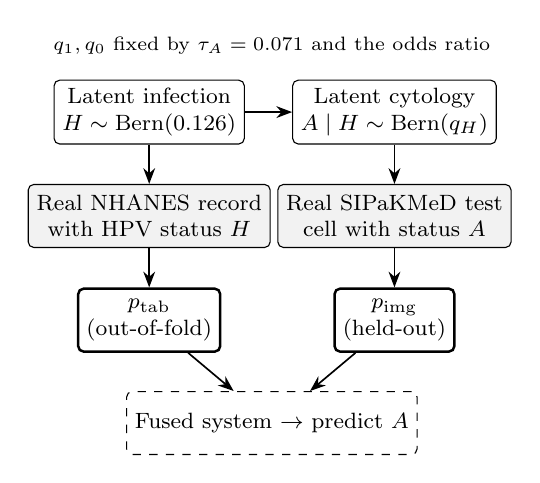
\begin{tikzpicture}[node distance=5mm and 6mm]
  \node[box] (h) {Latent infection\\$H\sim\mathrm{Bern}(0.126)$};
  \node[box, right=of h] (a) {Latent cytology\\$A\mid H\sim\mathrm{Bern}(q_H)$};
  \node[data, below=of h] (nt) {Real NHANES record\\with HPV status $H$};
  \node[data, below=of a] (ni) {Real SIPaKMeD test\\cell with status $A$};
  \node[model, below=of nt] (et) {$\ptab$\\(out-of-fold)};
  \node[model, below=of ni] (ei) {$\pimg$\\(held-out)};
  \node[op, below=9mm of $(et)!0.5!(ei)$] (f) {Fused system $\rightarrow$ predict $A$};
  \draw[arr] (h) -- (a); \draw[arr] (h) -- (nt); \draw[arr] (a) -- (ni);
  \draw[arr] (nt) -- (et); \draw[arr] (ni) -- (ei); \draw[arr] (et) -- (f); \draw[arr] (ei) -- (f);
  \node[font=\scriptsize, align=center, above=2mm of $(h.north)!0.5!(a.north)$] {$q_1,q_0$ fixed by $\tau_A=0.071$ and the odds ratio};
\end{tikzpicture}}
\caption{Construction of a semi-synthetic woman. Latent infection and cytology states are drawn from trial-matched margins, and each state selects a real held-out record from the corresponding data set. The fused system is scored on the latent cytology label $A$.}
\label{fig:synth}
\end{figure}

\emph{Image quality.} The real image expert is nearly perfect on this test set, so its ranking cannot be improved. To study settings with less certain image reads (e.g., poorer slides), we also added Gaussian noise to the image log-odds with a standard deviation chosen to give target AUROCs of 0.95, 0.90 and 0.80 ($\sigma=7.39$, 10.06 and 15.99). Each noisy expert was then re-calibrated by Platt scaling \cite{platt1999probabilistic} on image-only data drawn at its native prevalence, which is data that would also be available in practice.

\emph{Comparators.} We compared the raw image output; the image re-anchored by \eqref{eq:anchor}; the questionnaire pre-test risk \eqref{eq:bridge}; the naive mean and naive product of the raw expert outputs; the sum rule \cite{kittler1998combining} applied to the re-anchored and bridged probabilities; the proposed rule \eqref{eq:fuse} with and without the safety floor; and a \emph{paired-data oracle}, a logistic-regression stacker on $(\logit\pimg,\logit\ptab)$ trained on a separate synthetic cohort with known labels. The oracle is an upper-bound reference that requires paired training data, which do not exist in practice.

\emph{Experiments.} E1 crossed the odds ratio with image quality. E2 misspecified the link, with the true $\mathrm{OR}=10$ while the fusion assumed values from 1 to 100. E3 removed images and/or questionnaires at random from 0\% to 100\% of women. E4 applied conformal abstention at $\alpha\in\{0.01,0.05,0.10\}$, calibrated on a separate synthetic cohort. Each configuration used 20 replicates of 20,000 women (plus 20,000 for oracle training or conformal calibration). Two further analyses used real data only: CO-PRIOR re-anchoring of each expert under resampled deployment prevalences (20 resamples of 8,000 cases per prevalence), and per-expert conformal coverage over 50 random calibration/test splits.

%% =====================================================================
\section{Experimental Setup}
\label{sec:setup}

\subsection{What is evaluated on what}
Nothing is evaluated on data used to fit it. The cytology expert is scored on a fixed list of 504 test images that took no part in any gradient update (Protocol~A), and, in the robustness run, on 379 cells from slides that appear in no training image (Protocol~B). The questionnaire expert is scored only through out-of-fold predictions: every woman is scored by the one fold of the five that did not train on her, with imputation, scaling and isotonic calibration all refitted inside each fold. The fused system consumes exactly these held-out outputs; no expert is retrained at any point in the fusion experiments, and the fusion itself has no fitted parameters.

\subsection{Experiments}
Table~\ref{tab:experiments} lists the seven experiments, what each varies, and where the result appears. Experiments~1--3 use only real data. Experiments~4--7 use the semi-synthetic cohort of Section~\ref{sec:synthetic}, each as 20 independent replicates of 20,000 women; within a replicate every method sees the same women and the same expert outputs, so differences isolate the fusion rule. Experiments~4--7 were run twice in full, once with the Protocol~A image expert and once with the Protocol~B expert, giving the 56 configurations quoted in the results.

\begin{table}[t]
\caption{Experiments, How They Were Executed, and Where They Appear}
\label{tab:experiments}
\centering\footnotesize
\setlength{\tabcolsep}{3pt}
\begin{tabular}{@{}p{0.055\columnwidth}p{0.40\columnwidth}p{0.27\columnwidth}p{0.17\columnwidth}@{}}
\toprule
\# & Question and execution & Varied & Reported in \\
\midrule
1 & Cytology accuracy: one training run per protocol, scored on the fixed test set & Teacher vs student; Protocol A vs B & Tables~\ref{tab:image}, \ref{tab:grouped}; Figs.~\ref{fig:training}--\ref{fig:grouped} \\
2 & Questionnaire accuracy: 5-fold cross-validation, all preprocessing in-fold, 1,000 bootstrap intervals & Six classifier families & Table~\ref{tab:tabular}; Figs.~\ref{fig:tabmodels}--\ref{fig:tabimp} \\
3 & Calibration under prevalence shift: each expert's held-out predictions resampled to a target prevalence, 20 resamples & Deployment prevalence $\tau$; with/without re-anchoring & Fig.~\ref{fig:coprior} \\
4 & Conformal coverage: 50 random calibration/test splits per expert & Target coverage $1-\alpha$ & Fig.~\ref{fig:confreal} \\
5 & Fusion quality: nine rules scored on identical synthetic cohorts & Link odds ratio (1--100) $\times$ image quality (0.80--0.999) & Table~\ref{tab:fusion}; Figs.~\ref{fig:gain}, \ref{fig:headline}, \ref{fig:dca} \\
6 & Wrong epidemiological link: true odds ratio fixed at 10 & Assumed odds ratio (1--100) & Fig.~\ref{fig:misspec} \\
7 & Missing inputs: modalities deleted at random, routing returns what remains & Fraction without image / without questionnaire & Fig.~\ref{fig:missing} \\
\bottomrule
\end{tabular}
\end{table}

\subsection{Metrics}
Image metrics were accuracy, balanced accuracy, macro-F1, Cohen's $\kappa$, macro one-versus-rest AUROC, expected calibration error (ECE; 15 top-label bins for five classes and 10 bins for binary outputs \cite{guo2017calibration}) and Brier score, plus sensitivity and specificity for the binary collapse. Tabular and fusion metrics were AUROC, average precision, Brier score, ECE, sensitivity at 90\% specificity and net benefit from decision-curve analysis \cite{vickers2006decision}. Confidence intervals are percentile bootstrap intervals over 1,000 resamples of the held-out predictions \cite{efron1994bootstrap}.

\subsection{Implementation}
Everything ran on one workstation with a single NVIDIA RTX 5060 Ti (16~GB) under WSL2, using TensorFlow 2.21 with tf-keras, scikit-learn 1.8 \cite{pedregosa2011scikit}, LightGBM 4.7 and XGBoost 3.4. Training the teacher and distilling the student took 49 minutes for the slide-grouped run; the cross-validated questionnaire study, including permutation importance, took under two minutes on the processor; and the complete set of fusion experiments took under two minutes. Latency was measured after warm-up at batch size 1. Grad-CAM \cite{selvaraju2017gradcam} maps were computed on the last convolutional layer with respect to the pre-softmax score of the predicted class, because gradients of a saturated softmax vanish; the rebuilt forward pass was checked to reproduce the model's predictions exactly.

%% =====================================================================
\section{Results}

\subsection{Cytology expert}
\emph{Training (how it was run).} The teacher was trained once with the two-stage schedule of Section~\ref{sec:image}: 25 epochs with the backbone frozen, then 13 fine-tuning epochs before early stopping; the student was then distilled from the frozen teacher for 24 epochs. Fig.~\ref{fig:training} plots the per-epoch logs of those three runs on one axis, with the dotted line marking the moment the backbone was unfrozen.

Three things are visible. First, freezing the backbone gets the teacher only to about 0.93 validation accuracy, and unfreezing it lifts both curves to roughly 0.95, which is why the second stage is needed. Second, the student reaches 0.96 validation accuracy within 15 epochs, above its own teacher, so distillation is not merely compressing the teacher but regularising the smaller network. Third, the student's validation loss is orders of magnitude below its training loss and swings by two decades between epochs. That is an artefact of the objective in \eqref{eq:kd}: 90\% of the loss is the teacher-matching term, which the validation loss does not include, so the reported validation loss is a small residual cross-entropy on easy cells. Accuracy, not loss, is therefore the quantity to read for the student, and early stopping was set on validation accuracy for that reason.

\begin{figure*}[t]
\centering
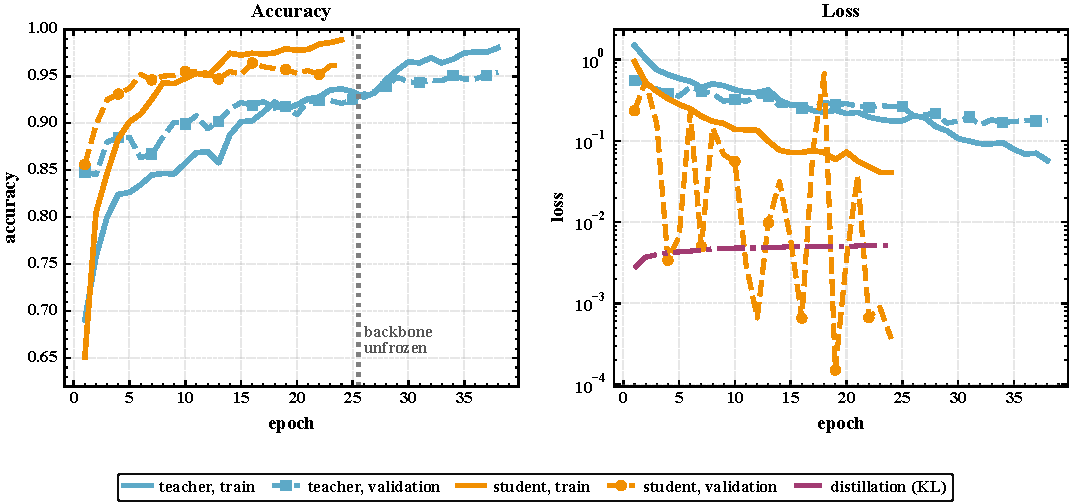
\includegraphics[width=\textwidth]{img_training}
\caption{Learning curves (Protocol~A), redrawn from the per-epoch logs. The teacher runs for 38 epochs (25 with the backbone frozen, then 13 fine-tuned; dotted line) and the student for 24 distillation epochs. Right: losses on a logarithmic scale, including the teacher-matching (KL) term.}
\label{fig:training}
\end{figure*}

\emph{Test performance.} On the fixed 504-image test set (Table~\ref{tab:image}), the student reached 96.4\% accuracy (95\% CI 94.6--98.0), macro-F1 0.965 and macro AUROC 0.998, matching the teacher (96.0\%, 0.961, 0.996) with 4.0 times fewer parameters (4.7 M vs 18.6 M), an 11.4-times smaller file and 2.4 times the throughput. Both models were well calibrated (ECE 0.020 and 0.024). For the binary collapse, the student separated abnormal from normal cells with AUROC 0.999, sensitivity 98.0\% and specificity 98.7\%. On the full 1,504-image held-out set the student reached 96.3\% accuracy (macro AUROC 0.997), confirming that the fixed test set is representative.

\begin{table}[t]
\caption{Cytology Expert on the Fixed SIPaKMeD Test Set ($n=504$, Protocol A)}
\label{tab:image}
\centering\footnotesize
\setlength{\tabcolsep}{4pt}
\resizebox{\columnwidth}{!}{%
\begin{tabular}{@{}lcc@{}}
\toprule
Metric & Teacher B4 & Student B0 \\
\midrule
Accuracy (95\% CI) & 0.960 (0.942--0.976) & \textbf{0.964} (0.946--0.980) \\
Balanced accuracy & 0.963 & \textbf{0.966} \\
Macro-F1 & 0.961 & \textbf{0.965} \\
Cohen's $\kappa$ & 0.950 & \textbf{0.955} \\
Macro AUROC (95\% CI) & 0.996 (0.992--0.998) & \textbf{0.998} (0.997--0.999) \\
ECE / Brier & 0.024 / 0.065 & \textbf{0.020} / \textbf{0.057} \\
\midrule
Abnormal vs normal AUROC & 0.997 & \textbf{0.999} \\
Sensitivity / specificity & \textbf{1.000} / 0.974 & 0.980 / \textbf{0.987} \\
\midrule
Parameters & 18.6 M & \textbf{4.7 M} \\
Model file & 224 MB & \textbf{19.6 MB} \\
Latency (batch 1) & 141.5 ms & \textbf{73.0 ms} \\
Throughput (batch 32) & 138 img/s & \textbf{334 img/s} \\
\bottomrule
\end{tabular}}
\end{table}

\emph{Which cells are confused (Fig.~\ref{fig:imgconf}).} Both models were run once over the fixed 504-image test set and their predictions tabulated against the true labels; rows are normalised so each entry is the fraction of a true class assigned to a predicted class, with raw counts in parentheses. Errors are not spread evenly. They concentrate in two places: between the two abnormal classes, and between metaplastic cells and the abnormal classes (the teacher sends 6\% of koilocytotic cells to dyskeratotic and 6\% of metaplastic cells to koilocytotic). Parabasal and superficial-intermediate cells are recognised almost perfectly (F1 0.979--0.995). This pattern is clinically benign for screening: the confusions lie \emph{within} the abnormal group, or between benign metaplasia and abnormality, which is the direction that triggers a second look rather than a missed lesion.

\emph{Ranking and the fusion input (Fig.~\ref{fig:imgroc}).} The left panel sweeps a threshold over each class score in a one-versus-rest manner; the right panel does the same after collapsing the five classes to the abnormal-versus-normal decision that the fusion actually consumes, $\pimg = P(\text{dyskeratotic}) + P(\text{koilocytotic})$. Every class curve is close to the upper-left corner (per-class AUROC 0.997--1.000), and the collapsed decision reaches 0.999 for the student. The collapsed panel is the one that matters downstream: it shows the image expert enters the fusion as an almost perfectly discriminating signal on this test set, which is why Section~\ref{sec:fusres} also studies deliberately weakened image experts.

\emph{Are the probabilities trustworthy (Fig.~\ref{fig:imgrel})?} Test cells were sorted by predicted $\pimg$ and split into twelve equal-count bins; each point plots the mean prediction in a bin against the observed fraction of abnormal cells in that bin. Points on the diagonal mean the stated probability matches reality. Both models track the diagonal closely (ECE 0.024 and 0.020), so the outputs can be treated as probabilities rather than scores. This is a precondition for the fusion, which manipulates these numbers with Bayes' rule; it is also why the miscalibration introduced later by prevalence shift (Section~\ref{sec:fusres}) is a property of the deployment population and not of the network.

\begin{figure*}[t]
\centering
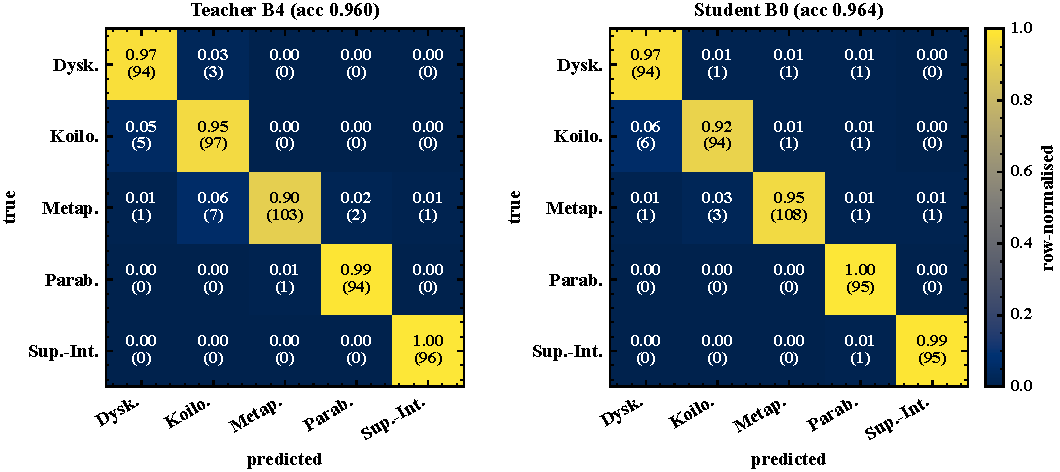
\includegraphics[width=\textwidth]{img_confusion}
\caption{Row-normalised confusion matrices on the fixed test set (counts in parentheses). Left: teacher. Right: student.}
\label{fig:imgconf}
\end{figure*}

\begin{figure*}[t]
\centering
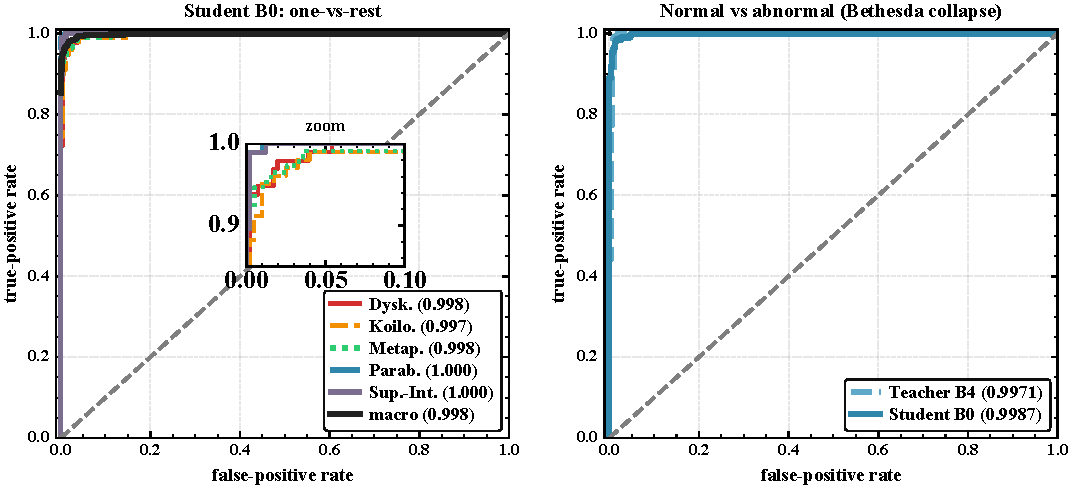
\includegraphics[width=\textwidth]{img_roc}
\caption{ROC analysis. Left: one-versus-rest curves of the student per class with the macro average (inset: zoom on the low false-positive region). Right: abnormal-versus-normal curves after the Bethesda collapse for teacher and student.}
\label{fig:imgroc}
\end{figure*}

\begin{figure}[t]
\centering
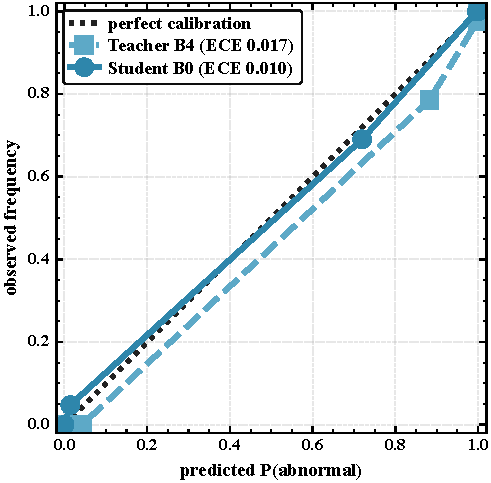
\includegraphics[width=\columnwidth]{img_reliability}
\caption{Reliability of the binary abnormality probability $\pimg$ on the test set (12 equal-count bins).}
\label{fig:imgrel}
\end{figure}

\emph{Where the networks look (Fig.~\ref{fig:gradcam}).} For one correctly classified test cell per class, we took the gradient of the pre-softmax score of the predicted class with respect to the last convolutional feature map, averaged it over space to weight the channels, summed the weighted channels, applied a rectifier and upsampled the result over the input cell. The rebuilt forward pass was verified to reproduce the model's own predictions exactly before any map was drawn, so the maps describe the deployed network and not an approximation of it. The maps give a mixed picture. For the teacher, the koilocytotic map forms a ring around the nucleus, where the koilocytic perinuclear halo lies, and the parabasal and superficial-intermediate maps cover the cell body and perinuclear cytoplasm; the dyskeratotic map, however, is weak and diffuse. The student's maps are more fragmented and partly fall on cell borders and background, although for the superficial-intermediate example they peak on both nuclei. Because the last convolutional feature map is only $12\times12$, these maps localise coarsely, and we treat them as a plausibility check rather than as evidence of cytological reasoning.

\begin{figure*}[t]
\centering
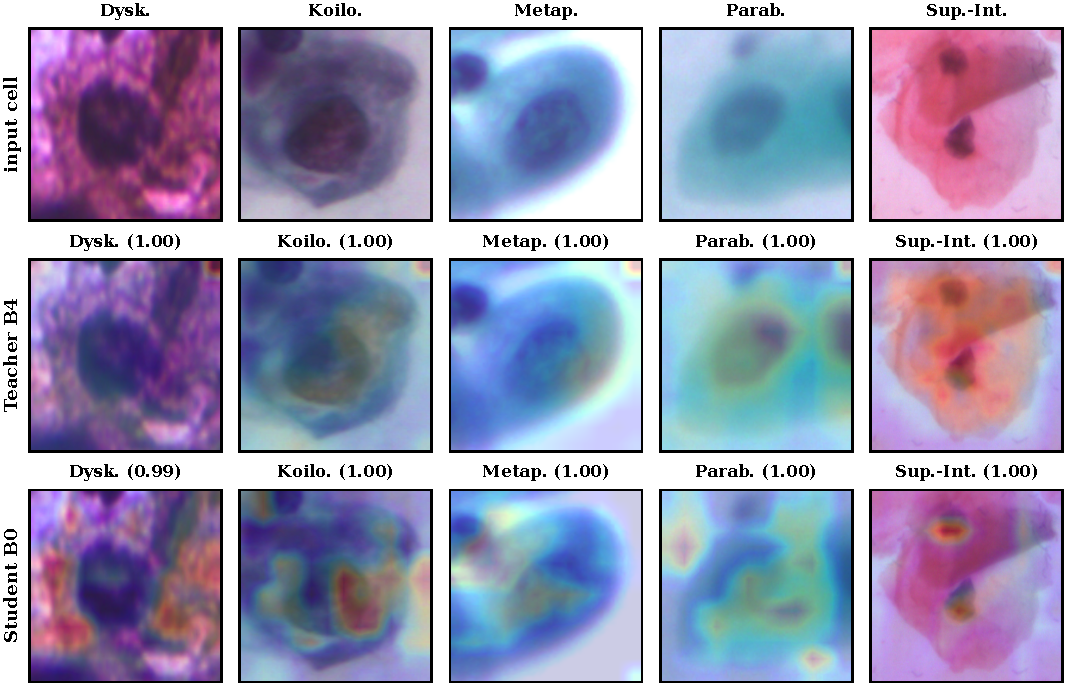
\includegraphics[width=\textwidth]{img_gradcam}
\caption{Grad-CAM (pre-softmax class score) for one correctly classified test cell per class. Top: input cell. Middle: teacher. Bottom: student. Each title gives the predicted class and its probability.}
\label{fig:gradcam}
\end{figure*}

\emph{Does slide overlap inflate the result (Fig.~\ref{fig:grouped})?} Under the random file-level split, 404 of the 414 cropped test cells (97.6\%) come from a slide that also contributed training images, so Protocol~A could in principle reward recognition of seen slides rather than of cell morphology. To measure that, we repeated the entire teacher--student recipe from scratch on the 4,049 cropped cells alone, assigning whole source slides within each class to training, validation and test, so that no test cell shares a slide with any training cell (2,819/851/379 cells). The left panel compares the student under the two protocols on the four headline metrics; the right panel is its confusion matrix on the unseen-slide test set. Performance remained high: the teacher reached \GTacc{} accuracy (95\% CI 0.955--0.989; macro AUROC \GTauc{}) and the student \GSacc{} (95\% CI 0.937--0.976; macro-F1 \GSfone{}, macro AUROC \GSauc{}, abnormal-versus-normal AUROC \GSbin{}, sensitivity 95.4\%, specificity 99.1\%). The student's accuracy fell by 0.6 percentage points relative to Protocol~A, within the confidence intervals, while the teacher's rose. Slide overlap therefore did not materially inflate the reported accuracy. The student's main remaining weakness on unseen slides is koilocytotic cells (recall 0.86), which are most often confused with metaplastic cells (Fig.~\ref{fig:grouped}, right). Protocol~B is the more conservative estimate of performance on new patients, and we repeat the fusion experiments with this student.

\begin{table}[t]
\caption{Effect of Slide-Level Separation on the Cytology Expert}
\label{tab:grouped}
\centering\footnotesize
\setlength{\tabcolsep}{3.5pt}
\resizebox{\columnwidth}{!}{%
\begin{tabular}{@{}lcccc@{}}
\toprule
Protocol / model & Acc. & Macro-F1 & Macro AUROC & Abn. AUROC \\
\midrule
A: random, teacher & 0.960 & 0.961 & 0.996 & 0.997 \\
A: random, student & 0.964 & 0.965 & 0.998 & 0.999 \\
B: slide-grouped, teacher & \GTacc & \GTfone & \GTauc & \GTbin \\
B: slide-grouped, student & \GSacc & \GSfone & \GSauc & \GSbin \\
\bottomrule
\end{tabular}}
\end{table}

\begin{figure*}[t]
\centering
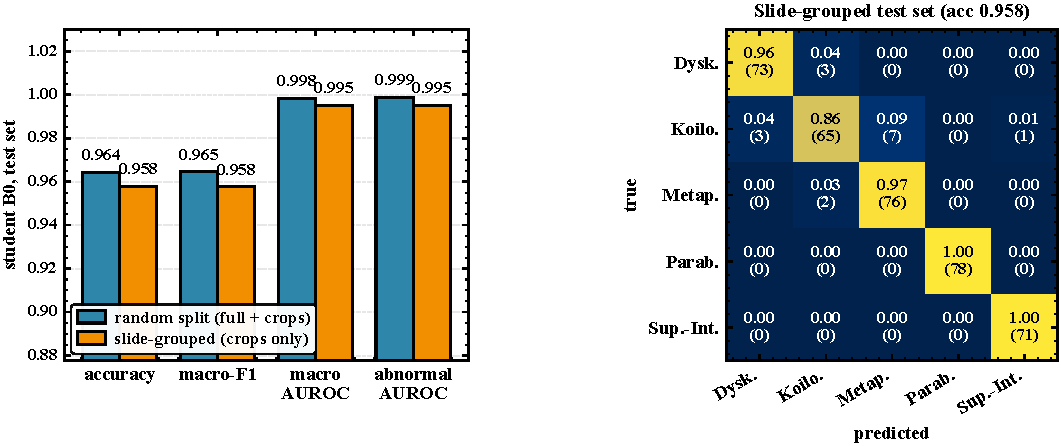
\includegraphics[width=\textwidth]{img_grouped}
\caption{Effect of slide-level separation. Left: student performance under the random file-level split (Protocol~A) and the slide-grouped single-cell split (Protocol~B). Right: row-normalised confusion matrix of the student on the slide-grouped test set ($n=379$ cells from unseen slides).}
\label{fig:grouped}
\end{figure*}

\subsection{HPV-risk expert}
\emph{Which model to deploy (Fig.~\ref{fig:tabmodels}).} Each of the six families was fitted five times, once per cross-validation fold, with imputation and scaling refitted inside every fold; each woman is scored by the fold that did not train on her, and the resulting out-of-fold probabilities are scored once. Error bars are 95\% bootstrap intervals over 1,000 resamples of those predictions, so overlapping bars mean the families are not distinguishable on this data. That is what the figure shows: logistic regression, random forest, LightGBM and XGBoost lie between 0.683 and 0.687 AUROC with fully overlapping intervals, and only $k$-nearest neighbours is clearly worse (0.624). The practical reading is that model capacity is not the limiting factor here, the available questionnaire items are; so we deploy the simplest and most inspectable family, logistic regression (AUROC 0.687, 95\% CI 0.676--0.697; PR-AUC 0.404 against a chance level of 0.246). Table~\ref{tab:tabular} lists the full metrics.

\emph{Turning scores into probabilities (Fig.~\ref{fig:tabcal}).} Class weighting makes the model behave as though positives and negatives were equally common, so its raw probabilities are systematically too high for a cohort that is 24.6\% positive; the raw curve accordingly sits far below the diagonal (ECE 0.227). Isotonic regression fitted in an inner three-fold loop, so that every calibrated probability is still out-of-fold, pulls the curve onto the diagonal (ECE 0.007) and improves the Brier score from 0.223 to 0.171 while leaving discrimination untouched (AUROC 0.686). Calibration is a prerequisite for this expert to enter the fusion at all, because \eqref{eq:bridge} multiplies its output by epidemiological rates; an uncalibrated score would corrupt that arithmetic. At a threshold equal to the cohort prevalence, the calibrated expert flags 68.1\% of infected women at 60.0\% specificity.

\begin{table*}[t]
\caption{HPV-Risk Expert: Stratified Five-Fold Cross-Validation on NHANES ($n=12{,}634$, 24.6\% High-Risk HPV Positive). Class Weighting, No Oversampling; Operating Point 0.5 for Accuracy, Sensitivity, Specificity and F1}
\label{tab:tabular}
\centering\footnotesize
\begin{tabular}{@{}lcccccccc@{}}
\toprule
Model & AUROC (95\% CI) & PR-AUC (95\% CI) & Brier & ECE & Accuracy & Sensitivity & Specificity & F1 \\
\midrule
Logistic regression & \textbf{0.687} (0.676--0.697) & 0.404 (0.387--0.422) & 0.223 & 0.227 & 0.642 & 0.631 & 0.646 & 0.464 \\
Random forest & 0.684 (0.674--0.695) & 0.396 (0.380--0.413) & \textbf{0.172} & \textbf{0.025} & \textbf{0.754} & 0.141 & \textbf{0.954} & 0.220 \\
LightGBM & 0.684 (0.673--0.695) & 0.408 (0.390--0.427) & 0.199 & 0.136 & 0.688 & 0.496 & 0.751 & 0.439 \\
XGBoost & 0.683 (0.672--0.693) & \textbf{0.409} (0.391--0.428) & 0.201 & 0.145 & 0.686 & 0.518 & 0.741 & 0.448 \\
Extra trees & 0.675 (0.664--0.685) & 0.376 (0.362--0.392) & 0.177 & 0.040 & 0.747 & 0.158 & 0.938 & 0.235 \\
$k$-nearest neighbours & 0.624 (0.612--0.634) & 0.325 (0.312--0.339) & 0.198 & 0.113 & 0.726 & 0.227 & 0.889 & 0.289 \\
\midrule
Logistic regression, isotonic & 0.686 & 0.402 & \textbf{0.171} & \textbf{0.007} & 0.620$^{\dagger}$ & \textbf{0.681}$^{\dagger}$ & 0.600$^{\dagger}$ & \textbf{0.468}$^{\dagger}$ \\
\bottomrule
\multicolumn{9}{@{}l}{$^{\dagger}$Operating point equal to the cohort prevalence (0.246).}
\end{tabular}
\end{table*}

\begin{figure*}[t]
\centering
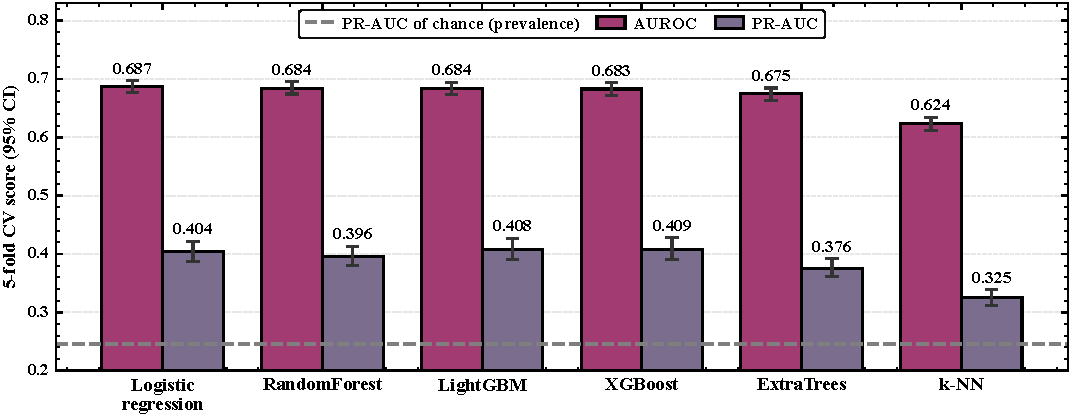
\includegraphics[width=\textwidth]{tab_models}
\caption{Cross-validated AUROC and PR-AUC (95\% bootstrap CIs) of the six classifier families. The dashed line is the PR-AUC of a chance classifier (prevalence).}
\label{fig:tabmodels}
\end{figure*}

\begin{figure}[t]
\centering
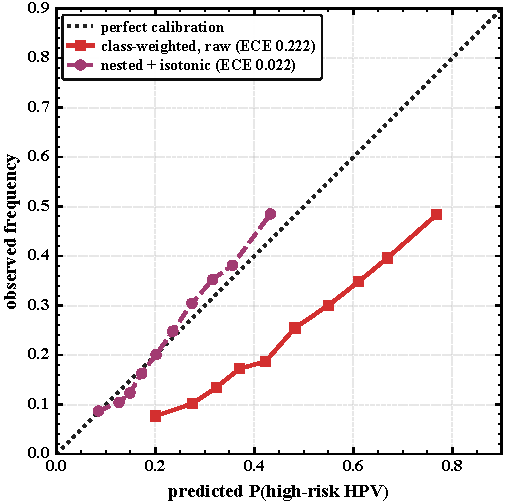
\includegraphics[width=\columnwidth]{tab_calibration}
\caption{Reliability of the logistic-regression expert before and after nested isotonic calibration (10 equal-count bins).}
\label{fig:tabcal}
\end{figure}

\emph{What the expert has learned (Fig.~\ref{fig:tabimp}).} Importance is measured by permutation: within each held-out fold, one feature at a time is shuffled five times and the drop in AUROC is recorded, so the bars report how much the model's ranking actually relies on a variable rather than how large its coefficient is. Bars are coloured by the sign of that variable's coefficient in the deployed model, with yes/no and serology items flipped so the colour always means the clinically intuitive direction.

The ranking is behavioural and demographic, not clinical: marital status (AUROC drop 0.045), smoking status (0.037), partners per sexually active year (0.023), lifetime smoking (0.018), age (0.014) and ever having had sex (0.012). The directions match HPV epidemiology: being unmarried, acquiring partners at a higher rate, being sexually active, testing positive for herpes simplex virus type-2 and being younger all raise the predicted risk, while later first intercourse and higher income lower it. Two cautions belong with this figure. The two smoking variables are strongly collinear, so their individual coefficient signs are unstable even though the pair is jointly informative; and these associations are correlational markers of exposure, not causes of infection. The value of the figure is that a screening service can see which answers drive a woman's risk score, and that none of them is a proxy for the outcome itself.

\begin{figure}[t]
\centering
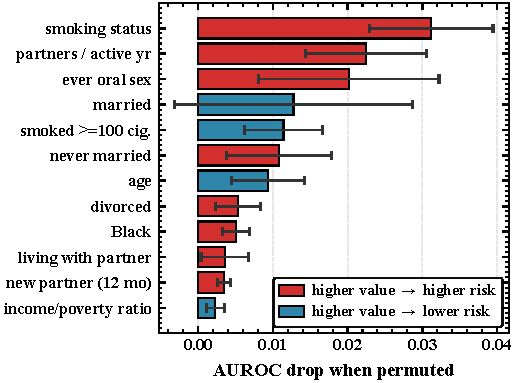
\includegraphics[width=\columnwidth]{tab_importance}
\caption{Permutation importance of the logistic-regression expert: mean AUROC drop on held-out folds ($\pm$1 SD across folds), top 15 features.}
\label{fig:tabimp}
\end{figure}

\subsection{Fused system}
\label{sec:fusres}
\emph{Prior re-anchoring on real data (Fig.~\ref{fig:coprior}).} This experiment uses no synthetic patients at all. For each target prevalence $\tau$ on the horizontal axis we resampled an expert's own held-out predictions, with replacement, into a cohort of 8,000 cases containing that fraction of positives, and measured the calibration error twice: on the raw probabilities, and after applying the re-anchoring of \eqref{eq:anchor}. Twenty resamples give the error bars. The figure therefore answers a question a screening service would ask before deploying either expert unchanged: what happens when the clinic's case mix differs from the training data? Without correction, the questionnaire expert's ECE rose from 0.011 at its training prevalence to 0.111 at the ATHENA infection prevalence (12.6\%) and to 0.209 at 2\%. With \eqref{eq:anchor} it stayed at or below 0.011 across the whole range from 2\% to 50\%. The image expert, which is sharper, degraded less (ECE 0.016 at 7.1\% prevalence), but re-anchoring still lowered its error at every low prevalence (0.007 at 7.1\%, 0.003 at 1\%).

\begin{figure*}[t]
\centering
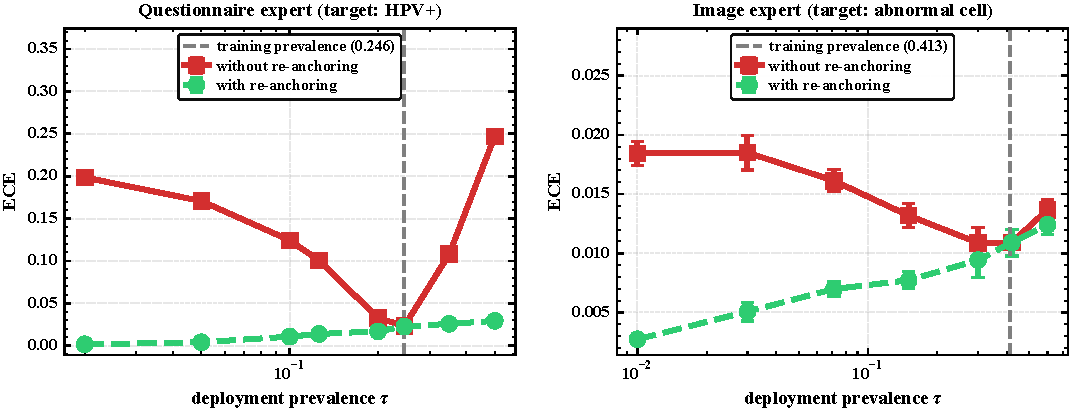
\includegraphics[width=\textwidth]{fus_coprior_real}
\caption{Calibration under prevalence shift on real held-out predictions. Each expert's predictions are resampled to a deployment prevalence $\tau$ (log scale) and scored with and without CO-PRIOR re-anchoring (mean $\pm$ SD over 20 resamples). The dashed line marks the training prevalence.}
\label{fig:coprior}
\end{figure*}

\emph{Conformal coverage on real data (Fig.~\ref{fig:confreal}).} Each expert's held-out predictions were split at random into a calibration half and a test half fifty times. On each split, class-conditional thresholds were computed on the calibration half at a target coverage $1-\alpha$ and applied to the test half; we recorded how often the true label fell inside the returned set (coverage) and how often the set was not a single class, in which case the system defers. Mondrian split-conformal prediction met its target for both experts. At a 90\% target, coverage was 0.902 for the questionnaire expert and 0.902 for the image expert. The price of that guarantee differs sharply: the weak questionnaire expert abstains on 63\% of women at 90\% coverage, while the image expert abstains on 10\% of cells. A questionnaire alone is therefore a triage signal that often defers, not a stand-alone screening decision.

\begin{figure*}[t]
\centering
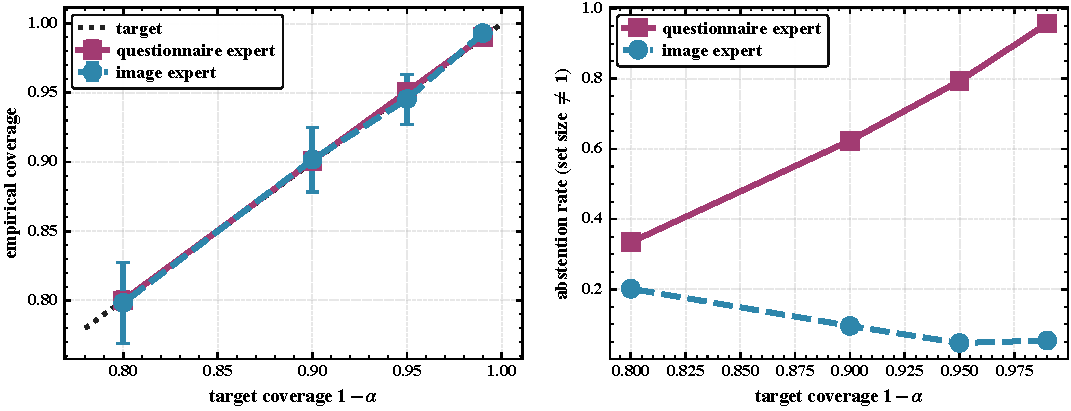
\includegraphics[width=\textwidth]{fus_conformal_real}
\caption{Per-expert split-conformal prediction on real held-out data (50 random calibration/test splits). Left: empirical versus target coverage. Right: abstention rate (prediction set not a singleton).}
\label{fig:confreal}
\end{figure*}

\emph{Fusion on the semi-synthetic cohort.} Every configuration below was run as 20 independent replicates of 20,000 synthetic women, each woman carrying a real held-out questionnaire record and a real held-out cell image selected by her latent state (Section~\ref{sec:synthetic}); reported values are means over replicates. Within a configuration all methods see exactly the same women and the same two expert outputs, so differences between rows are attributable to the fusion rule alone. Table~\ref{tab:fusion} reports the reference scenario ($\mathrm{OR}=10$, prevalence 7.1\%). Three findings hold across all settings.

(i) \emph{The unpaired rule matches the paired-data oracle and never harms.} Fig.~\ref{fig:gain} plots, for each fusion rule, the AUROC it adds to the image-only output as the infection--cytology link strengthens from none ($\mathrm{OR}=1$) to very strong ($\mathrm{OR}=100$), with one curve per image-expert quality; a value of zero means the questionnaire added nothing, and a negative value means fusing made matters worse. In the left panel the solid curves (proposed rule) sit on top of the dotted curves (the oracle stacker trained on paired data) everywhere: across all 28 combinations of link strength and image quality the two agree to within 0.0003 AUROC, and with an image expert of AUROC 0.90 the values were 0.9026 and 0.9025. Every solid curve also stays at or above zero, so the rule never degraded the image-only ranking. This is the paper's central empirical claim: the information a stacker would have extracted from paired patients is recoverable from the two marginal experts plus the epidemiological link, with no paired data at all.

(ii) \emph{Naive fusion is harmful.} The mean of the raw outputs lowered the AUROC relative to the image alone in 23 of the 28 settings (for example, 0.893 versus 0.900) and was badly miscalibrated in all of them (ECE 0.13--0.21). The sum rule fell below the image alone in 20 settings (Fig.~\ref{fig:gain}, right), and the naive product in every setting with $\mathrm{OR}\le10$; the product ranks reasonably when the link is strong but remains miscalibrated (ECE 0.06 at an image AUROC of 0.90) because it ignores both training priors.

(iii) \emph{Discrimination gains are small and conditional; calibration gains are large.} With the real image expert (AUROC 0.999), no method can improve the ranking. As image evidence weakens, the questionnaire's contribution grows with the strength of the infection--cytology link: the AUROC gain of the proposed rule over the image alone rose from $+0.0026$ ($\mathrm{OR}=10$) to $+0.0091$ ($\mathrm{OR}=100$) for an image AUROC of 0.90, and from $+0.006$ to $+0.022$ for an image AUROC of 0.80. The questionnaire's own AUROC for cytological abnormality is only 0.58 at $\mathrm{OR}=10$ and 0.65 at $\mathrm{OR}=100$, which bounds the achievable gain. By contrast, the raw image output was strongly miscalibrated at the 7.1\% screening prevalence (ECE 0.176 for an image AUROC of 0.90), and CO-PRIOR fusion reduced this to 0.004. Fig.~\ref{fig:headline} shows both facts side by side for the reference scenario: on the left the ROC curves of the single experts, the sum rule, the proposed rule and the oracle nearly coincide, confirming that little ranking is to be won; on the right the same predictions are binned and plotted against observed frequency, where the raw image curve departs from the diagonal by an order of magnitude at low risk while the proposed rule follows it. A woman assigned a 10\% risk by the raw image expert is not a 10\% risk in a screening population; after re-anchoring she is. Most of this correction comes from prior re-anchoring, which also benefits the image-only output. When the image expert is already near-perfect, all well-behaved methods are calibrated to within about 0.01, and the choice among them matters little.

\emph{Replication with the slide-grouped image expert.} Repeating every synthetic experiment with the Protocol~B student (real abnormal-versus-normal AUROC 0.995) gave the same conclusions. Across its 28 settings the proposed rule was again within 0.0003 AUROC of the paired-data oracle and never below the image alone, and naive averaging lowered the AUROC in 23 settings. In the reference scenario with an image AUROC of 0.90, the values were 0.9014 (proposed), 0.9013 (oracle), 0.8988 (image alone) and 0.8949 (sum rule), and re-anchoring reduced the image ECE from 0.172 to 0.004.

\begin{table}[t]
\caption{Fusion on the Semi-Synthetic Cohort (OR$\,=10$, Abnormality Prevalence 7.1\%; Mean of 20 Replicates of 20,000 Women). Sens@90 Is Sensitivity at 90\% Specificity}
\label{tab:fusion}
\centering\footnotesize
\setlength{\tabcolsep}{2.4pt}
\resizebox{\columnwidth}{!}{%
\begin{tabular}{@{}lcccccc@{}}
\toprule
& \multicolumn{2}{c}{Image AUROC 0.999} & \multicolumn{4}{c}{Image AUROC 0.90} \\
\cmidrule(lr){2-3}\cmidrule(l){4-7}
Method & AUROC & ECE & AUROC & ECE & Brier & Sens@90 \\
\midrule
Image, raw & 0.9987 & 0.016 & 0.9000 & 0.176 & 0.103 & 0.702 \\
Image, CO-PRIOR & 0.9987 & 0.007 & 0.9000 & 0.004 & 0.047 & 0.702 \\
Questionnaire, pre-test & 0.5799 & 0.002 & 0.5776 & 0.002 & 0.066 & 0.165 \\
Naive mean & 0.9927 & 0.130 & 0.8931 & 0.171 & 0.083 & 0.703 \\
Naive product & 0.9987 & 0.008 & 0.8975 & 0.064 & 0.058 & 0.695 \\
Sum rule (CO-PRIOR) & 0.9947 & 0.062 & 0.8955 & 0.040 & 0.051 & 0.705 \\
\textbf{CO-PRIOR fusion} & \textbf{0.9987} & \textbf{0.005} & \textbf{0.9026} & \textbf{0.004} & \textbf{0.046} & \textbf{0.709} \\
\quad + safety floor & 0.9987 & 0.006 & 0.9026 & 0.004 & 0.046 & 0.709 \\
\midrule
Paired-data oracle$^{\ast}$ & 0.9987 & 0.004 & 0.9025 & 0.004 & 0.046 & 0.708 \\
\bottomrule
\multicolumn{7}{@{}l}{$^{\ast}$Requires paired training data; reference only.}
\end{tabular}}
\end{table}

\begin{figure*}[t]
\centering
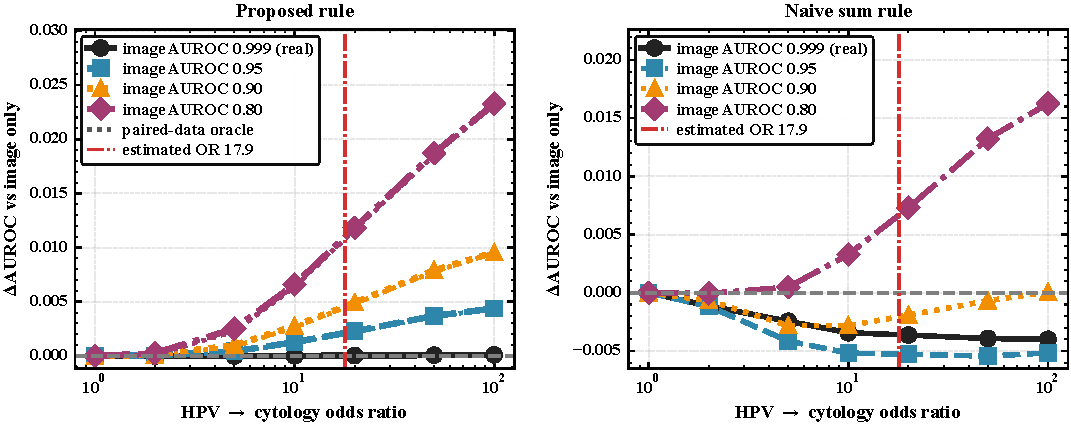
\includegraphics[width=\textwidth]{fus_gain_vs_or}
\caption{AUROC gain over the image-only output as a function of the infection--cytology odds ratio, for four image-expert qualities. Left: proposed CO-PRIOR fusion (solid) and the paired-data oracle (dotted), whose curves coincide. Right: the naive sum rule, which falls below the image alone when the link is weak.}
\label{fig:gain}
\end{figure*}

\begin{figure*}[t]
\centering
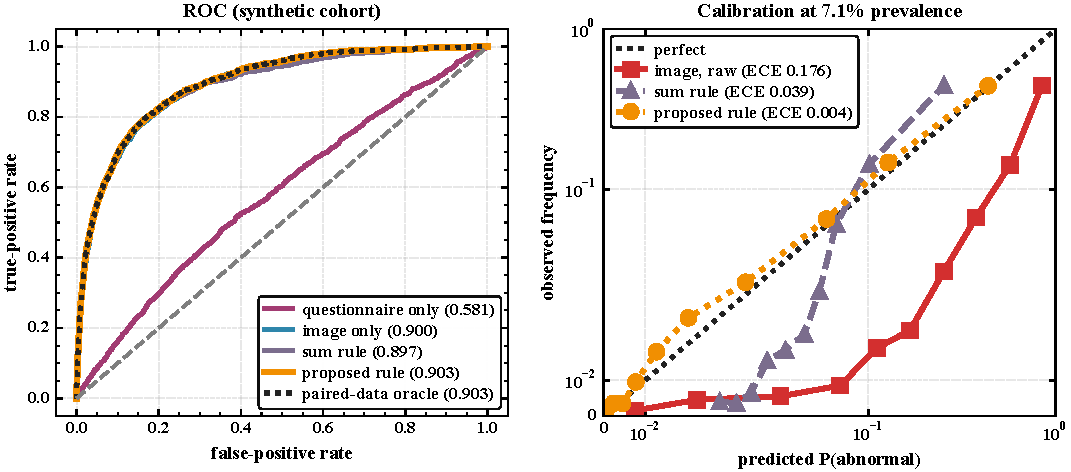
\includegraphics[width=\textwidth]{fus_headline_090}
\caption{Reference scenario ($\mathrm{OR}=10$, image AUROC 0.90). Left: ROC curves of the single experts, the sum rule, the proposed fusion and the paired-data oracle (AUROC in parentheses). Right: reliability at the 7.1\% screening prevalence (log-scaled axes).}
\label{fig:headline}
\end{figure*}

\emph{What if the assumed link is wrong (Fig.~\ref{fig:misspec})?} The fusion needs one external quantity, the odds ratio tying infection to abnormal cytology, and a service adopting it would have to take that number from the literature rather than measure it. To test the cost of getting it wrong, we generated cohorts with a true odds ratio of 10 and let the fusion assume values from 1 (no link) to 100 (very strong), a hundred-fold misspecification in either direction. For an image AUROC of 0.90 the AUROC stayed between 0.901 and 0.904 and the calibration error between 0.003 and 0.005. The rule degrades gracefully because the questionnaire enters only through a pre-test prior: assuming too weak a link shrinks that prior towards the population average, which reduces the fusion to the image-only answer rather than to a wrong one.

\begin{figure*}[t]
\centering
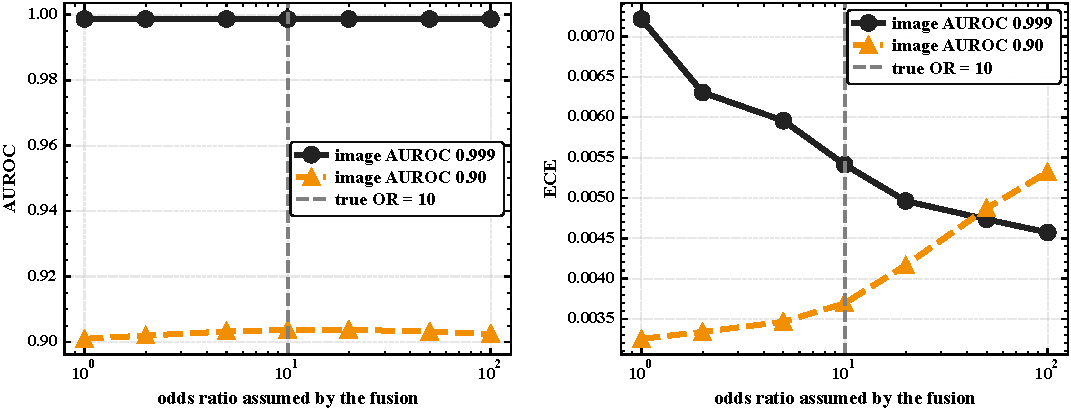
\includegraphics[width=\textwidth]{fus_misspec}
\caption{Misspecified epidemiological link. The true odds ratio is 10 (dashed); the fusion assumes the value on the horizontal axis. Left: AUROC. Right: ECE.}
\label{fig:misspec}
\end{figure*}

\emph{What if an input is missing (Fig.~\ref{fig:missing})?} Real screening data are incomplete: a woman may attend without a usable smear, or a smear may arrive without a questionnaire. We removed each modality independently at random from a given fraction of women (never both from the same woman) and let the routing of Section~\ref{sec:coprior} return whichever output remained available, then scored the whole cohort as one population. Each cell of the figure is the AUROC of that mixed population, so it measures the system as a service rather than the fusion rule in isolation. The output degrades smoothly as inputs disappear. With an image AUROC of 0.90, the AUROC fell from 0.903 with complete data to 0.854, 0.784 and 0.691 when 25\%, 50\% and 75\% of women had no image, and to 0.577 when only questionnaires were available. Removing questionnaires changed the AUROC by at most 0.002. Every woman nevertheless receives a calibrated estimate, and a woman without a smear still receives a meaningful pre-test risk.

\begin{figure}[t]
\centering
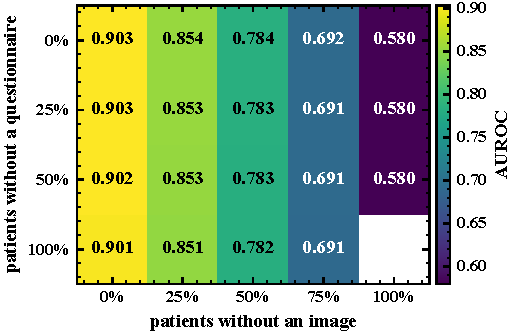
\includegraphics[width=\columnwidth]{fus_missing_090}
\caption{AUROC of the any-modality output when images and questionnaires are missing at random (image AUROC 0.90, $\mathrm{OR}=10$). Women never miss both inputs.}
\label{fig:missing}
\end{figure}

\emph{Abstention on the fused output.} Repeating the conformal procedure on the synthetic cohort, with thresholds calibrated on a separate cohort of the same size, the fused output achieved its nominal coverage (0.991, 0.950 and 0.900 at $\alpha=0.01$, 0.05 and 0.10). It deferred marginally fewer women than the image-only output (38.1\% versus 39.0\% at $\alpha=0.05$) while reaching 92.0\% accuracy on the cases it did answer. Adding the questionnaire therefore does not buy a meaningfully smaller deferral rate; the guarantee itself, and the ability to produce it for women with only one modality, is what the gate contributes.

\emph{Is the fused risk clinically useful (Fig.~\ref{fig:dca})?} Discrimination and calibration do not by themselves say whether acting on a score helps. For each referral threshold on the horizontal axis we therefore counted the women the system would refer, credited the true abnormal cases found and charged the false positives at the exchange rate implied by that threshold; the result is the net benefit, expressed in units of true cases per woman screened. Two default strategies bound the picture: refer everyone (dashed) and refer no one (dotted). Across the plausible range of referral thresholds the fused output lies at or above the image alone and well above both defaults, and the questionnaire alone is useful only at very low thresholds, where referring almost everyone is nearly free. This is the practical summary of the whole fusion experiment: the combined risk is never worse to act on, and it remains interpretable as a probability at the clinic's own prevalence.

\begin{figure}[t]
\centering
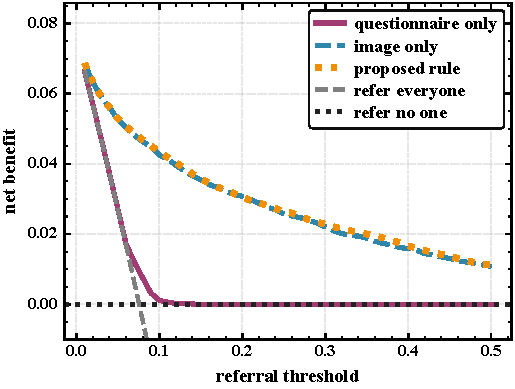
\includegraphics[width=\columnwidth]{fus_decision_090}
\caption{Decision curves for referral on the semi-synthetic cohort (image AUROC 0.90, $\mathrm{OR}=10$).}
\label{fig:dca}
\end{figure}

%% =====================================================================
\section{Discussion}
The main result is that two experts trained on disjoint populations can be combined into a single calibrated screening output without paired data, and that doing so correctly matters more than doing so at all. When the infection--cytology link is modelled explicitly and each expert's prior is removed, the unpaired combination recovers what a model trained on paired data would learn from the same two scores. This is expected under the conditional independence of \eqref{eq:fuse}, in which the Bayes-optimal combination has exactly this form, but it had not been demonstrated empirically for heterogeneous medical experts. Conversely, the fusion rules most often used in practice, averaging or multiplying probabilities, treat infection and abnormality as the same label and the two training priors as the same prior. Both assumptions are false here, and both cost discrimination and calibration.

The size of the benefit should be stated plainly. A questionnaire carries limited information about the cells on a slide: even in the strongest-link scenario, its AUROC for cytological abnormality is 0.65. When the cytology read is confident, fusion cannot and should not change it; the value of the questionnaire lies in the uncertain reads, in women for whom no smear is available, and in setting the pre-test risk that makes the final probability interpretable. The largest measured effect is calibration: a network trained on SIPaKMeD's 41\% abnormal cells reports probabilities that are far too high for a screening population with 7\% abnormal cytology, and prior re-anchoring corrects this without retraining. For clinicians this is the difference between a score that ranks women and a probability that can be compared with a referral threshold.

The distilled student is a practical choice for deployment: it matched or exceeded the teacher on every accuracy and calibration metric with a quarter of the parameters, about one-eleventh of the storage and 2.4 times the throughput, which suits screening settings with limited hardware. The HPV-risk expert reached the discrimination typically reported for questionnaire-based infection models; the families with the most flexibility did not outperform logistic regression, which suggests that the available items rather than the model limit performance. The strongest predictors, namely marital status, smoking, partner-acquisition rate and age, agree with established HPV epidemiology, which supports the plausibility of the learned risk.

The slide-grouped analysis shows why data-splitting protocols should be reported in detail. SIPaKMeD distributes cropped cells together with the fields they were cut from, and a random file-level split, as used in most published work on this data set, places related images on both sides of the split. In our case, holding whole slides out changed accuracy by less than the width of the confidence intervals, so the network appears to learn cell-level morphology rather than slide identity. Other architectures or training recipes may be more sensitive, and we recommend slide-grouped splits as the default. The fusion conclusions were identical with either image expert.

\subsection{Limitations}
\begin{itemize}
\item \emph{Semi-synthetic evaluation of fusion.} No real woman in this study has both an image and a questionnaire. The synthetic cohort uses real held-out records and trial-matched margins, but it assumes that the two records are independent given the latent state, and the infection--cytology link was swept rather than estimated from a paired population. A prospective paired cohort is needed to confirm the fused performance.
\item \emph{Single-cell images as a stand-in for a smear.} Each synthetic woman is represented by one cell image, whereas a real Pap smear contains thousands of cells. Slide-level aggregation (for example, multiple-instance learning) would be required in practice.
\item \emph{Endpoint and population differences.} The questionnaire expert predicts high-risk HPV in U.S. women aged 18--59 surveyed from 2003 to 2016, and HPV vaccination has since changed infection prevalence. Re-anchoring handles changes in prevalence but not changes in how risk factors relate to infection.
\item \emph{Image data.} SIPaKMeD is a single-source collection of conventional smears. Cross-data-set validation on collections with different staining and acquisition, harmonised through the Bethesda System, was not performed here and is the most important next step for the image expert.
\item \emph{Feature coding.} Nominal survey variables were used in their released integer coding; one-hot encoding might slightly improve the linear model.
\end{itemize}

%% =====================================================================
\section{Conclusion}
We showed that a cytology classifier and an HPV-risk questionnaire model, trained on data sets that share no patients, can be fused into a single calibrated, any-modality screening output. CO-PRIOR fusion removes each expert's training prior, bridges infection risk to cytological abnormality through an explicit epidemiological link, and treats the image as a likelihood ratio; a conformal gate defers uncertain cases. On a trial-anchored semi-synthetic cohort built from real held-out records, the unpaired rule matched a model trained on paired data, whereas naive fusion lowered discrimination and calibration. Its principal benefit is calibrated risk at screening prevalence, with modest discrimination gains that appear when cytology is uncertain. Validation on a prospective cohort in which both modalities are collected for the same women, and cross-data-set evaluation of the image expert, are the next steps towards clinical use.

\section*{Data and Code Availability}
SIPaKMeD and NHANES are publicly available. All evaluation scripts, fixed test-set lists, per-case predictions and figure-generation code used in this paper will be released with the article.

\clearpage   % flush every pending float before the references
\bibliographystyle{IEEEtran}
\bibliography{Mybib,refs_added}

\end{document}
